% XCircuit output "1.4b.tex" for LaTeX input from 1.4b.eps
\def\putbox#1#2#3#4{\makebox[0in][l]{\makebox[#1][l]{}\raisebox{\baselineskip}[0in][0in]{\raisebox{#2}[0in][0in]{\scalebox{#3}{#4}}}}}
\def\rightbox#1{\makebox[0in][r]{#1}}
\def\centbox#1{\makebox[0in]{#1}}
\def\topbox#1{\raisebox{-0.60\baselineskip}[0in][0in]{#1}}
\def\midbox#1{\raisebox{-0.20\baselineskip}[0in][0in]{#1}}
   \scalebox{1}{
   \normalsize
   \parbox{3.58333in}{
   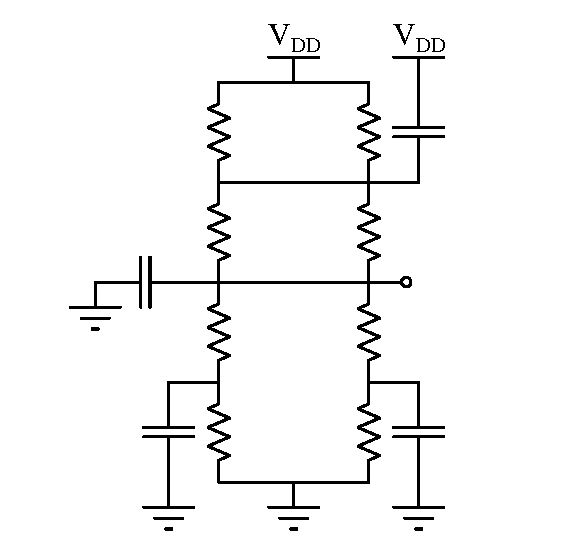
\includegraphics[scale=1]{1.4b.eps}\\
   % translate x=632 y=540 scale 0.38
   \putbox{2.93in}{2.62in}{1.20}{\(2C_gW_p\)}%
   \putbox{2.93in}{0.62in}{1.20}{\(\frac{C_gW_p}{2}\)}%
   \putbox{0.76in}{0.62in}{1.20}{\rightbox{\(\frac{C_gW_p}{2}\)}}%
   \putbox{1.18in}{1.95in}{1.20}{\rightbox{\(C_g(W_p+W_n)\)}}%
   \putbox{1.43in}{2.62in}{1.20}{$R_p$}%
   \putbox{1.43in}{1.95in}{1.20}{$R_p$}%
   \putbox{2.01in}{2.62in}{1.20}{$R_p$}%
   \putbox{2.01in}{1.95in}{1.20}{$R_p$}%
   \putbox{1.43in}{1.29in}{1.20}{$R_n$}%
   \putbox{2.01in}{1.29in}{1.20}{$R_n$}%
   \putbox{1.43in}{0.62in}{1.20}{$R_n$}%
   \putbox{2.01in}{0.62in}{1.20}{$R_n$}%
   } % close 'parbox'
   } % close 'scalebox'
   \vspace{-\baselineskip} % this is not necessary, but looks better
